%TODO Use lstinline instead of emph for code?

\chapter{Implementation}\label{chapter:Implementation}

The part of the sys-sage library implemented in this thesis enables users to share component subtrees or whole topologies between processes of a compute node by using shared memory regions.

To achieve this, all components of the given subtree, including its attruibutes and all DataPaths, are copied into a memory region shared between the involved processes.
The component tree and DataPath graph are then recreated in the memory of the receiving process.

\section{Capabilities and Usage}
If at any point during the lifetime of a sys-sage topology,

%\section{Limitations}
\section{Shared Memory}
The data sharing aspect of the implementation is realised using shared memory regions. These regions are created by opening files and mapping them using \emph{mmap()}. %TODO code styling?

\emph{mmap()} is a syscall that creates file backed memory mappings in the program's virtual address space that can be opened by multiple processes at once.
The mapped file can then be used just like any regular memory location. \cite{crotty22-mmap}

Using the \emph{MAP\_FIXED} flag when creating a \emph{mmap()} backed memory location will guarantee the virtual memory addresses to be equal across processes.
However, if the necessary memory location is not available in the current process, the mapping will fail, which could potentially have a major impact on the reliability of the library,
depending on the total available memory and its current utilization. [Quote manpage mmap] %TODO

Consequently, the \emph{MAP\_FIXED} flag is not used for the purposes of this thesis to achieve higher reliability when sharing component trees between processes.
As a result, the virtual memory addresses of the shared regions are not identical across processes.

Due to this, sharing pointers to addresses in the shared memory region between processes will not work, as the as the referenced location will have a different address in another process.
Instead, offset based pointers have to be used to reference shared memory locations.

In the sys-sage shared memory implementation, all offsets for pointers are calculated relative to the top of the shared region.
While this might not be possible for more general uses of offset pointers, as the start of the memory location might not always be known,
it is practical for the particular use-case of this thesis, since  memory regions are always handled as a whole and importing only parts of a shared component tree is not supported.

Calculating the offsets based on a shared, fixed location has the advantage that the offset pointers can be used more similarly to regular pointers and don't need to be recalculated when shared.
This means the location of components or DataPaths within the shared memory region can be compared or referenced without amiguity or confusion about the base of the offset.

The lifetime of the shared memory region is handled by a \emph{SharedMemory} object, as shown in \autoref{lst:sharedmemory}.

%TODO Wrap in Figure?
\begin{lstlisting}[language=c++, numbers=left, caption=SharedMemory Class, captionpos=b, label={lst:sharedmemory}]
    class SharedMemory {
      public:
        void* mem;
        char* cur;
        size_t size;
        ...

        SharedMemory(std::string path, size_t size);
        SharedMemory(std::string path);
        ~SharedMemory() { munmap(mem, size); }

      private:
        std::string path;
    };
\end{lstlisting}

Apart from the \emph{path} and \emph{size} size variables, which are used mainly in the creation and destruction of the shared memory region,
the \emph{SharedMemory} class consists of two pointers, \emph{mem} and \emph{cur}.
The \emph{mem} pointer always points to the top of the memory region, whereas the \emph{cur} pointer marks the current location to write or read from while importing or exporting a topology.

When a shared memory region is first created by the process sharing the topology, the path to the file used in the mapping as well as the total size needed have to be known.
The allocated size is then written to the start of the mapped file, to be read by other processes when importing the topology.
The file-backed memory region can then be used to export the topology until the \emph{SharedMemory} destructor is called and the file is unmapped using \emph{munmap()}.

The process importing the topology then uses the constructor in line 9 of \autoref{lst:sharedmemory}, which opens and maps the previously created file,
reads the total size of the data as written by the first process and then remaps the file to that size.
This has the advantage that the total size of the shared topology is always known to the importing process, without having to be provided seperately.
To share a topology, only the path to the memory mapped file needs to be provided, all other information can be read from the file, which simplifies the API and makes it easier
for users to share topologies without much inter-process comunication needed.


[Size Calculation]%TODO

\section{Components}
Topologies consist mainly of \emph{components}, which are organized as a hierarchical tree structure.
Each component represents a certain part of the hardware such as a CPU or cache.
Depending on the type of hardware the component represents, there are different subclasses of Components that can store specific hardware information such as the size of a cache.
Although there is no formal requirement, the top of the component tree is usually represented by a component of class \emph{Topology}, a subclass of \emph{Component},
which stores no additional values.
\autoref{lst:component_class} shows part of the sys-sage component class implementation.

\begin{lstlisting}[language=c++, numbers=left, caption=Component Class, captionpos=b, label={lst:component_class}]
    class Component {
      public:
        map<string, void*> attrib;

      protected:
        int id;
        string name;

        const int componentType;
        vector<Component*> children;
        Component* parent { nullptr };
        vector<DataPath*> dp_incoming;
        vector<DataPath*> dp_outgoing;
    };
\end{lstlisting}

As shown in \autoref{lst:component_class}, the component tree structure is created by the vector of component pointers in line 10 for the children, as well as a component pointer
for the parent.
Apart from that, the \emph{componentType} variable indicates, which component subclass and therefore which type of hardware is represented by the component.
\emph{Id} and \emph{name} store additional information to identify the component and underlying hardware.

The \emph{attrib map} enables users to attach arbitrary data to a component by associating it with a key string. This allows for a high degree of customization,
as the user can attach any data and update it dynamically as needed.

The vectors \emph{dp\_incoming} and \emph{dp\_outgoing} in lines 12 and 13 are used to store pointers to DataPaths associated with the component.

\subsection{Exporting Components}\label{subsection:export_components}
To export the topology into the shared memory region, the component tree structure including all \emph{attribs} and DataPaths needs to be transformed into one contiguous memory block.

Copying the component tree into the shared memory region is performed as follows:
\begin{enumerate}
    \item Determining the size of the component based on its \emph{componentType}.
    \item Copying the \emph{Component} object into the shared region using \emph{memcpy()} and the size determined previously.
    \item Copying the \emph{attrib} map.
    \item Copying the \emph{children} vector.
    \item Recursively copying the children.
\end{enumerate}

\begin{figure}[!ht] %TODO Fix position
    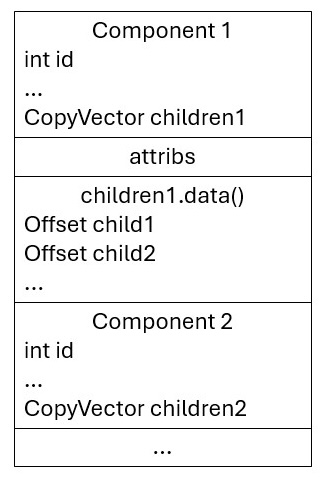
\includegraphics[scale=0.15]{images/component_memory.jpg} %TODO Replace graphic
    \centering
    \caption{Component Tree in Shared Memory}
    \label{figure:component_memory}
\end{figure}

\autoref{figure:component_memory} illustrates how the component tree is transformed into a single contiguous memory segment.
The \emph{Component} object is copied first, followed by its \emph{attribs} and the data segment of the \emph{children} vector.
It is important to note that the component pointers of the \emph{children} vector need to be replaced with the respective offsets of the children in the shared memory region,
as the virtual memory addresses will be different in each process.

To achieve this, the children are recursively exported and their offsets written to the \emph{children} vectors data array.

\subsection{Copying Vectors}
Since vectors use a pointer to the contiguous heap memory location storing the underlying data, simply copying the vector object into the shared memory region will not work,
as the virtual memory address of the data will be different in other processes. [FIND QUOTE] %TODO

To circumvent this issue, the components \emph{children} vector needs to be replaced with an offset based equivalent before being copied.
This is done by overwriting the vector object with a \emph{CopyVector} object as shown in \autoref{lst:copyvector}.

\begin{lstlisting}[language=c++, numbers=left, caption=Component Class, captionpos=b, label={lst:copyvector}]
    struct CopyVector {
        size_t offset;
        size_t size;
    };
\end{lstlisting}

The \emph{CopyVector} struct consists of an \emph{offset} and a \emph{size} variable that are used to reference the underlying data of the original vector.
\emph{Offset} stores the offset of the vector's data relative to the start of the shared memory region, while \emph{size} stores the number of elements in the vector.

While recreating the component in the importing process, the \emph{CopyVector} can simply be replaced by a regular vector again, using the copied data by resolving the offset and size.

\subsection{Importing Components}
Since the component tree is transformed into a single contiguous memory block, simply using \emph{memcpy()} to import the topology into the processes private memory will not work.

Importing the component tree into the receiving processes memory is done as follows:

\begin{enumerate}
    \item Reading the \emph{Components} \emph{componentType} to determine its type.
    \item Recreating the \emph{Component} using the copy constructor of the correct component subclass.
    \item Recreating the \emph{attrib} map by inserting all copied key-value pairs.
    \item Recursively copying the children and recreating the \emph{children} vector.
\end{enumerate}

To recreate the \emph{children} vector, the offsets of the children stored in the \emph{CopyVector}, as described in \autoref{subsection:export_components},
need to replaced with pointers to their respective memory addresses in the importing process.

\section{Attribs}
Components and DataPaths have an \emph{attrib} map that stores key-value pairs that can be used to add arbitrary data of any size.
It is implementated as a \lstinline{std::map<std::string, void*>}, mapping strings to 
\section{DataPaths}